% Created 2026-09-18 Fri 13:28
% Intended LaTeX compiler: pdflatex
\documentclass[presentation, aspectratio=169]{beamer}

\usepackage[utf8x]{inputenc}
\usepackage[T1]{fontenc}
\usepackage{graphicx}
\usepackage{longtable}
\usepackage{wrapfig}
\usepackage{rotating}
\usepackage[normalem]{ulem}
\usepackage{amsmath}
\usepackage{amssymb}
\usepackage{capt-of}
\usepackage{hyperref}
\usepackage{palatino}
\usepackage{tikz}
\usetikzlibrary{positioning,fit,backgrounds,arrows.meta}
\usetheme[numbering=fraction, progressbar=frametitle]{metropolis}
\author{Lucas Mello Schnorr, Vinicius Garcia Pinto, Raymond Namyst, Samuel Thibault}
\date{CARLA 2026 Advanced Tutorial}
\title{Introduction to Task-Based Parallel Programming with StarPU}
\subtitle{Session 1 — Foundations}
\begin{document}

\setbeamertemplate{navigation symbols}{}
\maketitle
\section{Overview}
\label{sec:org529c798}

\begin{frame}[label={sec:org01010fe}]{Where we're going today}
\begin{itemize}
\item \alert{Session 1 (now)}: the task-based paradigm, and how StarPU implements
it — no code yet, just the mental model.
\item \alert{Session 2}: your first StarPU programs, from a plain sequential
vector scale to task-based, partitioned matrix addition.
\item \alert{Session 3}: heterogeneous CPU/GPU codelets, and seeing what actually
happened with execution traces (StarVZ).
\end{itemize}
\end{frame}
\section{Why task-based programming?}
\label{sec:org7389c94}

\begin{frame}[label={sec:org9e8236b}]{Building a parallel application}
Some questions you face when starting to parallelize an application:
\begin{itemize}
\item How do I \alert{partition} the work and the data?
\item How do the pieces \alert{communicate}?
\item How do I \alert{map} pieces onto CPUs/accelerators/nodes?
\item If I later add a GPU, or move to a bigger cluster — do I rewrite
everything?
\end{itemize}
\end{frame}
\begin{frame}[label={sec:org67305d1}]{The trouble with "classical" parallel programming}
With MPI / OpenMP / CUDA written directly:
\begin{itemize}
\item \alert{You} decide, in the code, which core or device runs what, and when.
\item Adding a new kind of resource (a GPU, a second node) usually means
touching the core logic again.
\item Load balancing across heterogeneous, unequal resources becomes your
problem, by hand.
\end{itemize}
\end{frame}
\begin{frame}[label={sec:org80cfba1}]{A different strategy: describe the work, not the schedule}
Task-based programming (also called \alert{dataflow scheduling}):
\begin{itemize}
\item The application is split into well-defined \alert{tasks}.
\item The program's structure is submitted to a \alert{runtime system} as a
\alert{DAG} (Directed Acyclic Graph) of tasks and data dependencies.
\item The \alert{runtime} — not your application code — decides scheduling and
data movement, and can optimize both.
\end{itemize}
\end{frame}
\begin{frame}[label={sec:org8225b74}]{Advantages and disadvantages}
\begin{block}{Advantages}
\begin{itemize}
\item Less parallel-programming complexity exposed to the application.
\item The runtime can apply optimizations you didn't have to hand-code.
\item Adding a new kind of resource is (mostly) the runtime's problem.
\end{itemize}
\end{block}
\begin{block}{Disadvantages}
\begin{itemize}
\item One more layer of complexity: the runtime itself.
\item You give up some direct control over execution.
\item Behavior can be harder to predict (it depends on runtime decisions).
\end{itemize}
\end{block}
\end{frame}
\section{The structure of a task-based application}
\label{sec:org45f60b1}

\begin{frame}[label={sec:org5da7824}]{Three ingredients}
Every task-based application, represented as a DAG, is built from:
\begin{enumerate}
\item \alert{Tasks}
\item \alert{Data blocks}
\item \alert{Dependencies}
\end{enumerate}
\end{frame}
\begin{frame}[label={sec:org0310d82}]{Tasks}
A \alert{unit of computation} — usually sequential code, or a kernel meant to
run on an accelerator.
\begin{itemize}
\item Operates on well-defined data blocks.
\item Can have \alert{multiple implementations} (e.g., one for CPU, one for GPU).
\end{itemize}

Examples:
\begin{itemize}
\item Multiplying two tiles (blocks) of a matrix.
\item Applying one step/equation of a simulation model.
\end{itemize}
\end{frame}
\begin{frame}[label={sec:orgb7c935f}]{Data blocks}
A \alert{subdivision of the problem's data domain}.
\begin{itemize}
\item Used as input and/or output of tasks.
\item Each block can be read and/or written by different tasks.
\end{itemize}

Examples:
\begin{itemize}
\item Sub-blocks (tiles) of a matrix.
\item A subset of elements being simulated.
\end{itemize}
\end{frame}
\begin{frame}[label={sec:org24107bb}]{Dependencies between tasks}
Dependencies arise from tasks \alert{sharing the same data}.
\begin{itemize}
\item A task of type A produces data consumed by two tasks of type B.
\end{itemize}

\begin{center}
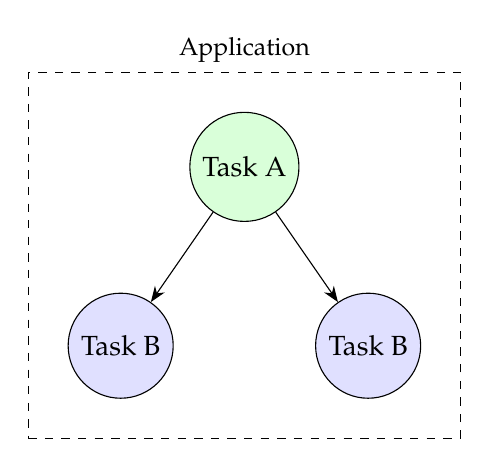
\begin{tikzpicture}[
  taskA/.style={circle, draw, fill=green!15, minimum size=1.1cm},
  taskB/.style={circle, draw, fill=blue!12, minimum size=1.1cm},
]
\node[taskA] (a) {Task A};
\node[taskB, below left=1.3cm and 0.6cm of a] (b1) {Task B};
\node[taskB, below right=1.3cm and 0.6cm of a] (b2) {Task B};
\draw[-{Stealth[length=2mm]}] (a) -- (b1);
\draw[-{Stealth[length=2mm]}] (a) -- (b2);
\begin{scope}[on background layer]
\node[draw, dashed, fit=(a)(b1)(b2), inner sep=0.5cm, label=above:{\small Application}] {};
\end{scope}
\end{tikzpicture}
\end{center}
\end{frame}
\begin{frame}[label={sec:org9fba9df}]{Turning a problem into tasks — is it always easy?}
Discretizing an algorithm/problem into tasks and data:
\begin{itemize}
\item Similar in spirit to the classic PCAM model (Partitioning,
Communication, Agglomeration, Mapping).
\item Not every algorithm is a natural fit — but that does not mean an
efficient task-based formulation doesn't exist; it may just take
more thought to find.
\end{itemize}
\end{frame}
\begin{frame}[label={sec:orgf9a0df3}]{Worked example: finding the largest element}
\begin{block}{The problem}
Given a vector of elements, find the largest one.
\end{block}
\begin{block}{What we need to figure out}
\begin{itemize}
\item What could a \alert{task} be?
\item What could the \alert{data} be?
\item What \alert{dependencies} result from that choice?
\end{itemize}
\end{block}
\end{frame}
\begin{frame}[label={sec:orgc04bcdb},fragile]{Worked example — the task}
 \alert{Task}: find the largest value in a sub-vector.
\begin{itemize}
\item Takes a vector of size \(N\).
\item Produces: the largest element.
\item Call it \texttt{MD3} ("max of 3").
\end{itemize}
\end{frame}
\begin{frame}[label={sec:orgc50d1be},fragile]{Worked example — the data}
 \alert{Data}: sub-vectors of the original vector, each of size \(N\).
\begin{itemize}
\item For this example, we pick \(N = 3\).
\item The \alert{outputs} of several \texttt{MD3} tasks can themselves be grouped into a
new sub-vector.
\end{itemize}
\end{frame}
\begin{frame}[label={sec:orgcafa4fa},fragile]{Worked example — the dependencies}
 Given a vector of 27 elements, we can run \texttt{MD3} nine times.
\begin{itemize}
\item That produces 9 distinct results.
\item Those 9 results can be grouped into 3 new sub-vectors of size 3.
\item We can apply \texttt{MD3} again on those results — and so on, recursively.
\end{itemize}
\end{frame}
\begin{frame}[label={sec:orga567137}]{Worked example — the execution graph}
\begin{center}
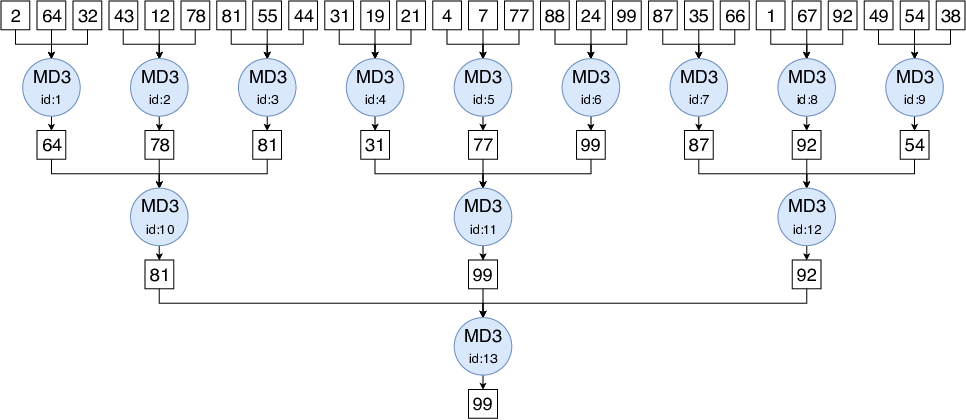
\includegraphics[width=0.9\linewidth]{./img/exemplo_dag_1.png}
\end{center}
\end{frame}
\begin{frame}[label={sec:org4bd4767}]{Worked example — the DAG}
\begin{center}
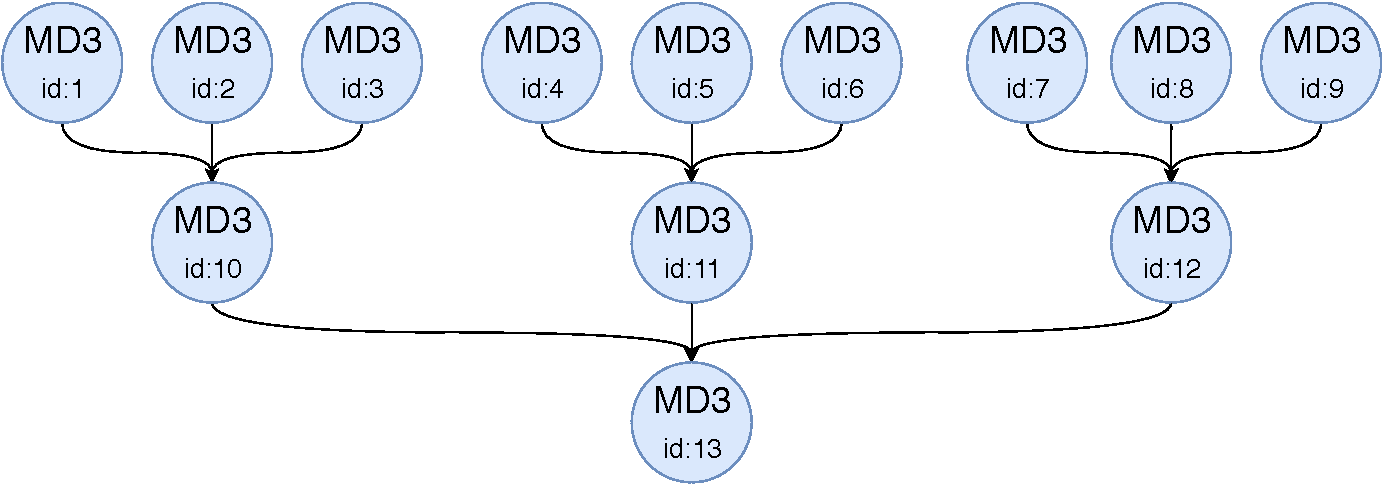
\includegraphics[width=0.9\linewidth]{./img/exemplo_dag_2.pdf}
\end{center}
\end{frame}
\begin{frame}[label={sec:orge3411d8}]{Worked example — where's the parallelism?}
Tasks that do \alert{not} share data, and whose dependencies are already
satisfied, can run concurrently.

\begin{center}
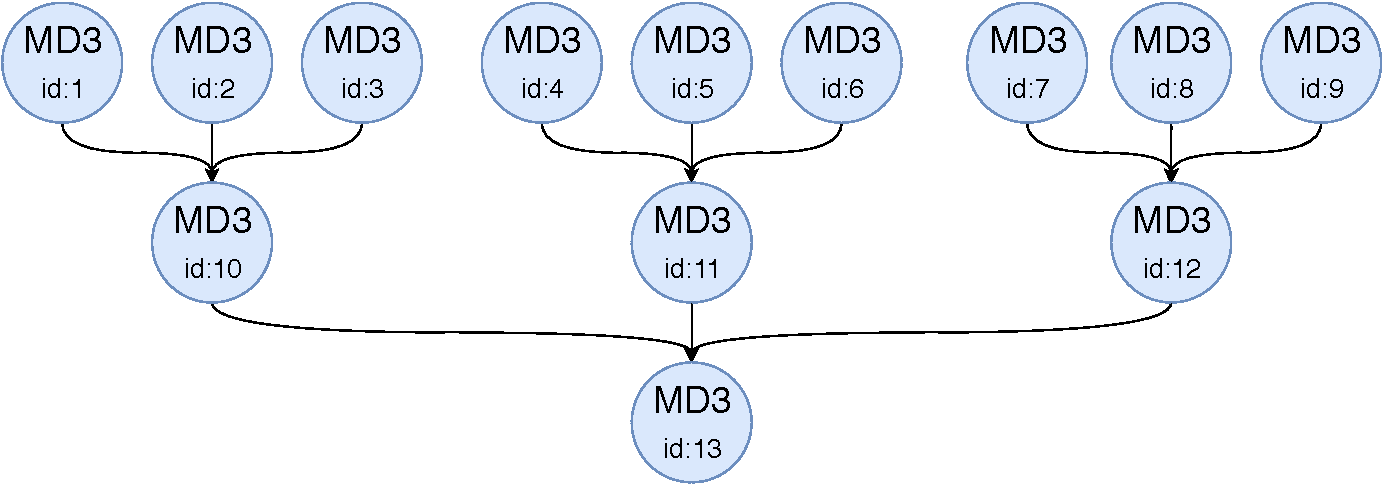
\includegraphics[width=0.9\linewidth]{./img/exemplo_dag_2.pdf}
\end{center}
\end{frame}
\section{Runtimes}
\label{sec:org94cb74a}

\begin{frame}[label={sec:orgd921a54}]{What is a runtime, here?}
A \alert{runtime system} executes the DAG you described, instead of you
scheduling it by hand.

Widely used in HPC already:
\begin{itemize}
\item OpenMP, MPI
\end{itemize}

Runtimes specifically built around task graphs:
\begin{itemize}
\item PaRSEC, OmpSs, OpenMP (tasking, >=4.0), XKaapi, \alert{StarPU}
\end{itemize}
\end{frame}
\begin{frame}[label={sec:org39e7c8a}]{What do you gain, what do you lose?}
\begin{block}{Advantages}
\begin{itemize}
\item Automatic scheduling decisions based on the DAG.
\item Automatic mapping of tasks to resources.
\item Automatic discovery of parallelism opportunities.
\item Automatic data movement between memories.
\end{itemize}
\end{block}
\begin{block}{Disadvantages}
\begin{itemize}
\item Runtime \alert{overhead}.
\item Reduced direct control over execution.
\end{itemize}
\end{block}
\end{frame}
\section{The StarPU runtime}
\label{sec:org2f18891}

\begin{frame}[label={sec:orge9d5538}]{What is StarPU?}
A general-purpose, task-based runtime system.
\begin{itemize}
\item Targets parallel applications on heterogeneous, multicore machines.
\item Developed at Université de Bordeaux / Inria.
\item C/C++/Fortran interface for submitting tasks onto resources.
\end{itemize}
\end{frame}
\begin{frame}[label={sec:org17a1477}]{Where StarPU sits in the software stack}
\begin{center}
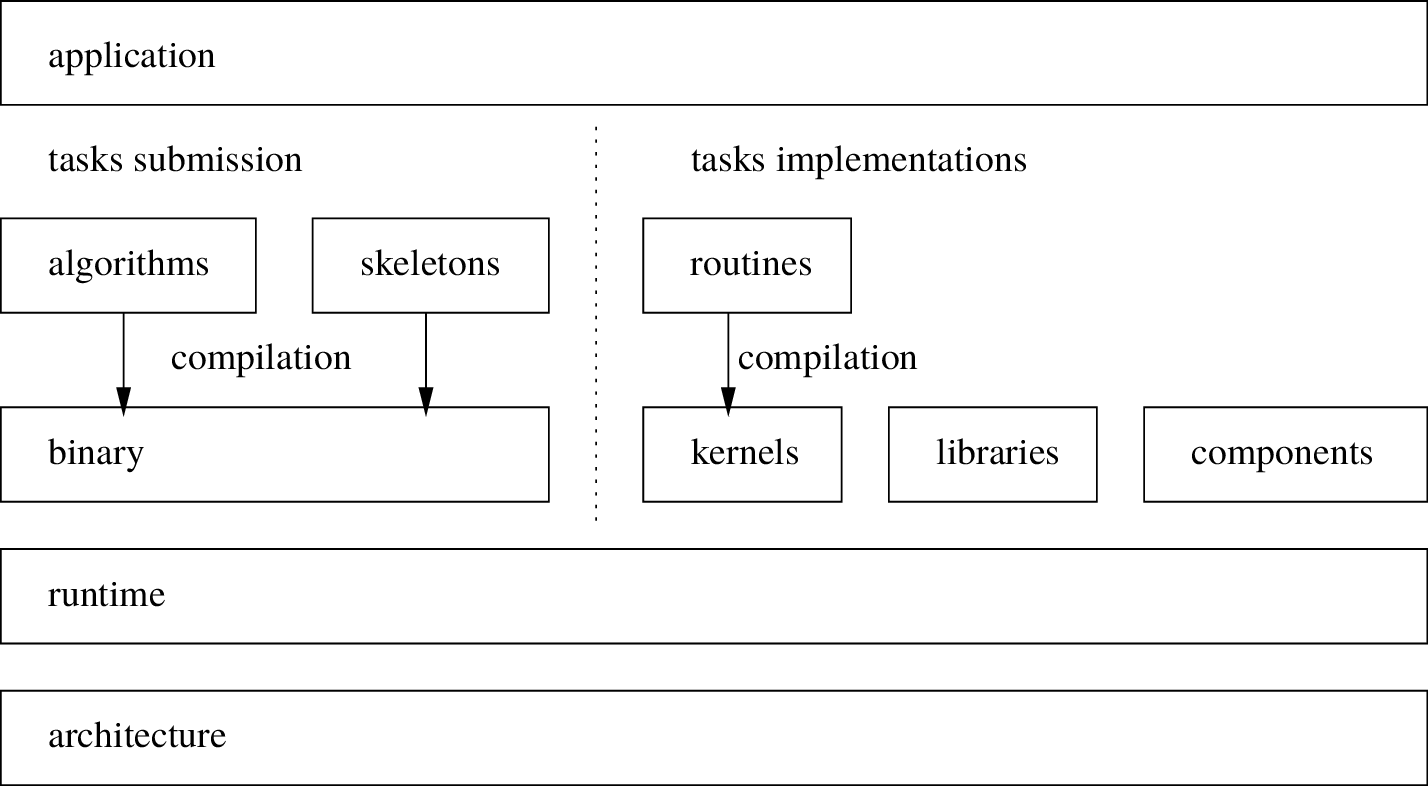
\includegraphics[width=0.85\linewidth]{./img/starpu_modelo.png}
\end{center}

\scriptsize
\center
Adapted from Thibault, 2018
\end{frame}
\begin{frame}[label={sec:org9b0e7d7}]{The STF model}
StarPU uses the \alert{Sequential Task Flow} (STF) model:
\begin{itemize}
\item The application submits tasks \alert{sequentially, as it runs}; the runtime
schedules them onto resources \alert{dynamically}.
\item The whole DAG does \alert{not} need to be known in advance.
\item Tasks can be submitted gradually, as execution proceeds.
\end{itemize}
\end{frame}
\begin{frame}[label={sec:org07469d4}]{Workers}
A \alert{worker} is the processing entity that actually executes a task.
\begin{itemize}
\item Each computing resource has one or more workers.
\end{itemize}

\begin{center}
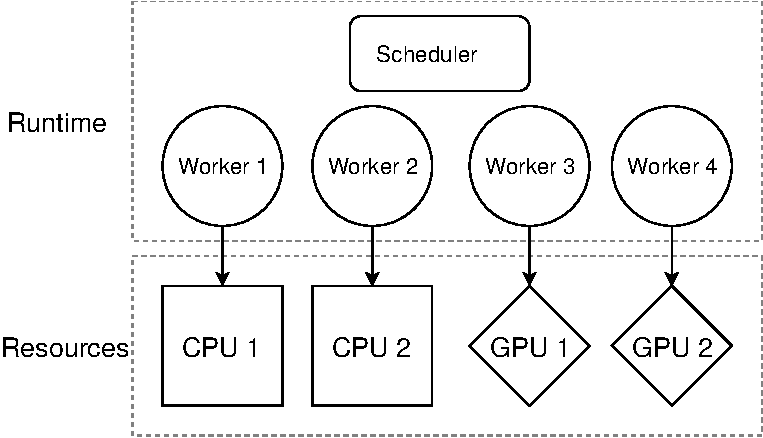
\includegraphics[width=0.5\linewidth]{./img/runtime.pdf}
\end{center}
\end{frame}
\begin{frame}[label={sec:org2462de0}]{Implementations and codelets}
Heterogeneous resources need different implementations of the same
task.
\begin{itemize}
\item Tasks are structured as \alert{codelets}, which may hold one implementation
per resource type (CPU, CUDA, OpenCL, \ldots{}).
\item \alert{Which} implementation actually runs is decided by the runtime, at
execution time.
\end{itemize}

(This is exactly what you will extend by hand in Session 3.)
\end{frame}
\begin{frame}[label={sec:org54d77b7}]{How StarPU structures a task-based program}
\begin{itemize}
\item Tasks are described as \alert{codelets}.
\item Memory blocks are described as \alert{data handles}.
\item Dependencies are computed \alert{implicitly}, from data reuse and
submission order — you do not write them explicitly.
\end{itemize}

(This is exactly what you will build by hand in Session 2.)
\end{frame}
\begin{frame}[label={sec:org1d93e08},fragile]{Scheduling strategies}
 Several schedulers are available, selectable at runtime:
\begin{itemize}
\item \texttt{lws} — local work-stealing
\item \texttt{eager} — single centralized task queue
\item \texttt{dm} — deque model, based on the HEFT heuristic
\item \texttt{dmda} — deque model, data-aware
\end{itemize}

Selected via the \texttt{STARPU\_SCHED} environment variable — no code change
needed to try a different one.
\end{frame}
\begin{frame}[label={sec:org525b1e0}]{Analyzing performance}
StarPU applications can be analyzed using execution \alert{traces}:
\begin{itemize}
\item The FxT format records fine-grained runtime events.
\item Traces can be converted to other formats (e.g. Paje) for
visualization.
\end{itemize}

\begin{center}
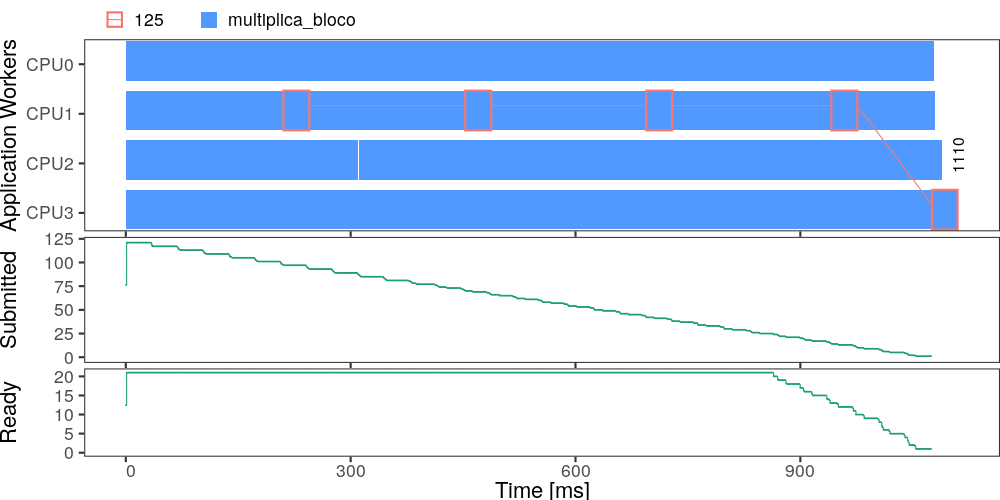
\includegraphics[width=0.5\linewidth]{./img/starvz.png}
\end{center}

This is exactly what Session 3, Part B, walks you through with StarVZ.
\end{frame}
\section{Wrap-up}
\label{sec:org585713c}

\begin{frame}[label={sec:org042d551}]{What's next}
You now have the vocabulary for Session 2:
\begin{itemize}
\item \alert{Codelet}, \alert{data handle}, \alert{task}, implicit \alert{dependency}.
\end{itemize}

In Session 2 you will:
\begin{enumerate}
\item Read and run three progressively richer StarPU programs.
\item Write a partitioned block-matrix-addition program from a skeleton.
\end{enumerate}

Questions before the break?
\end{frame}
\end{document}
